\newcommand{\mcX}{\mathcal{X}}
\newcommand{\bfitr}{\symbfit{r}}
\newcommand{\bfitc}{\symbfit{c}}

\chapter{Optimal Transport}\label{chap:optimal-transport}

In most decisions pertaining to life and sciences, the \textquote{shortest path} approach acts as the guiding strategy. Whenever a commodity, a person, a single bit of information, or any entity that is available at a given point and needs to be sent to a target point, one should ideally favour a way that uses the least effort possible. Typically, one would achieve this by moving an entity along a straight line from point A to point B on a plane.
The theory of \textbf{optimal transport} (OT) generalises that intuition in the case where, instead of moving only item at a time, we are concerned with the problem of simultaneously moving several items (or a distribution) from one configuration onto another.

As vacation planners can attest, planning the transportation for a group of individuals involved in the event, with the added constraint that they reach a given target configuration upon arrival, is considerably more tortuous than carrying it out for a single individual. In fact, thinking in terms of groups or rather distributions requires more advanced mathematical thinking and formalism, which was first explored by \textcite{monge1781memoire}. Regardless of how complicated this formalism might be, it has deep rooted connections to our daily life. 
Transportation, whether it be of people, goods, or information, rarely involves moving items. All major problems in economics, such as supply chain logistics, production planning, or warehousing, involve moving distributions, and that motif consistently appears in all seminal references on optimal transport.

\samptr{} uses an optimal transport based module in the fine-tuning phase to \textquote{transport} the support set embeddings into the domain of the query set embeddings. 
The transportation step \textquote{moves} the support embeddings in such a way that they overlap more areas of the query embedding domain, more specifically, we are trying to align the support embedding distribution with the query embeddings.
This transportation step is followed by prototypical classification which makes use of the \textit{transported support} embeddings. Using the transported support embeddings allows to create prototypes that are more representative of the items they are archetypes of.

\section{A brief historical context of Optimal Transport}\label{sec:ot-history}

The inception of optimal transport began in the late $18\textsuperscript{th}$ century under the rule of Louis \RN{16}, around $1781$, almost a decade before the French revolution of $1789$. The French physicist and mathematician Gaspard Monge\footnote{\url{https://mathshistory.st-andrews.ac.uk/Biographies/Monge/}} was the first to formulate the mathematical problem of \textquote{Excavation and embankments} (\citetitle{monge1781memoire}) - how to transport soil during the construction of forts and roads with minimal transport expenses. But what does shoveling dirt have to do with AI, statistics, or machine learning? Interestingly, the framework devised by \citeauthor{monge1781memoire} provides a formulation for comparing probability distributions.
Let us think of probability density functions as piles of dirt, where the \textquote{height} of the pile corresponds to the probability density at that point, and the shoveling of dirt between the piles as moving probability from one point to another, at a cost proportional to the distance between these two points.

The modern form of optimal transport and the one that is in use today in various applications was first formulated by the nobel laureate Leonid Vitaliyevich Kantorovich\footnote{\url{https://www.nobelprize.org/prizes/economic-sciences/1975/kantorovich/biographical/}}, the father of linear programming. 
It was his work in \citeyear{Kantorovich42} which cast the transportation as a probablistic measure on a metric space $\mcX$, where in a measure $\alpha$ is the intial one that needs to be transported to the second and final measure $\beta$, that is, the desired distribution after transportation. A transportation plan, as it is called by \citeauthor{Kantorovich42}, is also some probability measure $\pi$ on the Cartesian product of the space with itself $\mcX \times \mcX$.
We shall go into a bit more depth in later sections of this chapter.

It would be several years later that this theory was rediscovered because of the work of \textcite{Brenier1991PolarFunctions} and others that this theory provided a crucial basis for research, with strong links to convexity, partial differential equations, and statistics. Today, researchers in computer science disciplines, imaging, and more generally data scientists recognise that optimal transport theory grants powerful tools to study distributions in an abstract context, such as comparing readily available distributions.

\section{Discrete Optimal Transport}\label{sec:discrete-ot}

Since our work mostly deals with atomic items, we chose to focus on the discrete formulation instead of the continuous formulation, although it must be noted that the concepts spoken about here do not change drastically in the continuous domain.

\subsection{Asssignment Problem}\label{ssec:ot-assignment-prob}
\begin{figure}[ht]
    \centering
    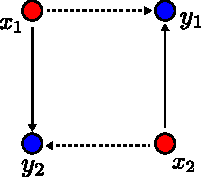
\includegraphics{chapters/assets/ot/monge1.pdf}
    \caption{Non-unique assignments. The other solution is dashed. Image sourced from \parencite{peyre2019computational}.}
    \label{fig:ot-non-uniq}
\end{figure}
In its most basic form, OT can be viewed as an assignment problem between sets of entities, that is, among all possible configurations, which is the best? This question is quite restrictive in the sense that we can only work with two sets of the same total size, that is, an \textit{initial} set and a \textit{target} set.

Each set can be represented as a histogram (or vector) $\bfitr$, that belongs to the probability simplex - the components of the vector sum up to $1$:
\begin{equation}
    \bfitr \in \left\{ x = (x_1, …, x_N) \in \mathbb{R}^N : \sum_{i=1}^N x_i = 1 \right\} 
    \label{eqn:r-simplex-defn}
\end{equation}

If we consider $\symbf{C}_{i,j}$ as the cost of moving an element from $i$ to $j$, then the quantity we wish to minimise is $\sum_{i} \symbf{C}_{i,\sigma(i)}$ , where $\sigma$ is a \textbf{permutation} of the set $\{1,\ldots, N\}$. This permutation represents an assignment of the bin $i$ of the first histogram to the output positions $j$ in the second histogram.

In this form optimal transport is fundamentally a combinatorial problem, and may be summarised as: 
How can we assign every element $i \in \{1, \ldots, N\}$ to elements $j \in \{1, \ldots, N\}$ in order to minimise $\sum_{i} \symbf{C}_{i,\sigma(i)}$.

The result of this search is called \textbf{optimal assignment}. As you may have already guessed, there can be $N!$ possible solutions to this problem; therefore, as $N$ grows, this problem quickly becomes intractable.
An important aspect is that this assignment is not unique. \Cref{fig:ot-non-uniq} is an example where two elements are assigned to two other elements that together form the four corners of a square.

\subsection{Working with Asymmetric Distributions}\label{ssec:ot-assym}

Requiring two equally sized histograms is a very strong constraint, hardly any real-world problems present themselves in this manner. By expanding the previous problem definition to a broader class of histograms, we obtain the Monge problem. In this version of the problem, several points $\bfitx_i$ can map to the same $y_j$ and their weights will be summed.

\begin{figure}[h]
    \centering
    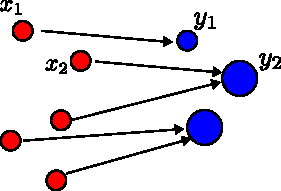
\includegraphics{chapters/assets/ot/monge2.pdf}
    \caption{The Monge problem. Image from \parencite{peyre2019computational}.}
    \label{fig:ot-assym}
\end{figure}

In this case, the mapping between inputs and outputs is no longer a combinatorial permutation, but a \textbf{surjective} map $\pi$. If points $\{\bfitx_1, \ldots, \bfitx_n\}$ have weights $\bfitr=\left(r_1, \ldots, r_n\right)$ and points $\left\{y_1, \ldots, y_m\right\}$ have weights $\bfitc=\left(c_1, \ldots, c_m\right)$, $\pi$ must verify:
\begin{equation}
    \forall j \in\{1, \ldots m\}, \quad c_{j}=\sum_{i: \pi\left(x_{i}\right)=y_{j}} r_{i}
    \label{eqn:ot-mass-conserv}
\end{equation}

\begin{tcolorbox}[title=Surjective functions]
A surjective function is a function $f$ that maps an element $\bfitx$ to every element $y$; that is, for every $y$, there is an $\bfitx$ such that $f(\bfitx) = y$. In other words, every element of the function's codomain is the image of at least one element of its domain. It is not required that $\bfitx$ be unique; the function $f$ may map one or more elements of $X$ to the same element of $Y$. 
\end{tcolorbox}

Even with this formulation, it does not make our job easier, the mass conservation constraint stated in \Cref{eqn:ot-mass-conserv} must be satisfied, while our problem still remains an assignment problem. We are still assigning element $\bfitx_i$ to element $\symbfit{y}_j$.

\subsection{The Kantorovich relaxation}\label{ssec:ot-kantorovich-relax}

Even with the above extension, this formulation of the optimal transport problem is still too constrained to be practically useful in many cases. As alluded to earlier in \Cref{sec:ot-history}, in 1942 \citeauthor{Kantorovich42} was instrumental in making OT viable for practical use. Kantorovich introduced a key idea, which is to \textbf{relax} the deterministic portion of the transportation. Points in the source histogram (or domains or distributions), $\bfitx_i$, no longer have to map to a single target point and can be \textit{fragmented} into \textit{partial} assignments, this is called \textbf{mass splitting}.

\begin{tcolorbox}[title=Relaxation]
Relaxation refers to the modelling strategy in mathematical optimisation and associated fields. Relaxation stands to be the approximation in relation to the difficult problem with regard to a nearby problem which stands to be easy to compute/solve.
\end{tcolorbox}

This new relaxed formulation is much more suitable for real-world situations, such as logistical problems. \textcite{hitchcock1941distribution} stated a version of this problem as follows:
When several factories supply a product to a number of cities, we seek the least costly means of distribution. Due to freight rates and other expenses, the cost of a ton of product to a particular city will vary according to the factory that supplies it and will also vary from city to city.
\begin{figure}[ht]
    \centering
    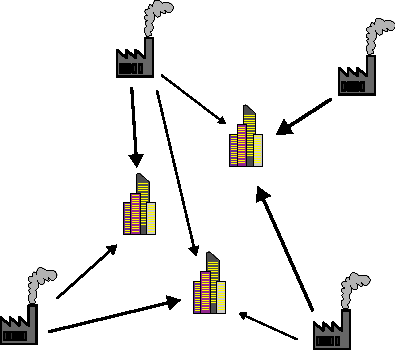
\includegraphics{chapters/assets/ot/logistic.pdf}
    \caption{Factories with different supply capacities have to deliver goods to cities with various demands.}
    \label{fig:ot-factories}
\end{figure}

To reflect this change, we will slightly modify our previous formulation by replacing the permutation function $\sigma$ by a coupling matrix $\symbf{\pi} = \symbf{\pi}_{i j} \in \mathbb{R}_{+}^{n \times m}$. In \Cref{fig:ot-factories}, each $\symbf{\pi}_{i j}$ would be the weight of the arrow from factory $i$ to city $j$.
As we have mentioned earlier, $\bfitr$ is a probability simplex, the same is applicable to $\bfitc$. With this established, all possible assignments can be written as:
\begin{equation} 
\label{eqn:ot-def}
\symbf{\Pi}(\bfitr, \bfitc)=\left\{\symbfit{\pi} \in \mathbb{R}_{+}^{n \times m} \mid \symbfit{\pi} \symbf{1}_{m}=\bfitr, \symbfit{\pi}^{\top} \symbf{1}_{n}=\bfitc\right\}.
\end{equation}

$\symbf{\Pi}(\bfitr, \bfitc)$ contains all non-negative $n \times m$ matrices for which all rows sum up to $\bfitr$ and all columns sum up to $\bfitc$. 
This makes $\symbf{\Pi}(\bfitr, \bfitc)$ a \textbf{polytope} of $\bfitr$ and $\bfitc$, representing a polyhedral set of $n \times m$ matrices.
$\symbf{\Pi}(\bfitr, \bfitc)$ is then essentially a collection of \textbf{transport plans} (coupling matrix) of which some are better than others.
Keep in mind that both $\bfitr$ and $\bfitc$ can only be accessed through a finite set of samples each, in \Cref{fig:ot-factories} that means a limited set of factories and cities.

\begin{tcolorbox}[title=Polytope]
The word polytope is used to mean a number of related, but slightly different, mathematical objects. A convex polytope may be defined as the convex hull of a finite set of points that are always bounded. \textquote{Convex} implying that there is a minimum point.
\end{tcolorbox}

\textcite{cuturi2013sinkhorn} also gives a probabilistic interpretation for $\symbf{\Pi}(\bfitr, \bfitc)$: for $A$ and $B$ two multinomial random variables taking values in  $\{\bfitx_1, \ldots, \bfitx_n\}$ and  $\{\symbfit{y}_1, \ldots, \symbfit{y}_m\}$ each with distribution $\bfitr$ and $\bfitc$, respectively, the set $\symbf{\Pi}(\bfitr, \bfitc)$ contains all possible \textit{joint probabilities} of $(A, B)$. Any matrix $\symbfit{\pi} \in \symbf{\Pi}(\bfitr, \bfitc)$ can be identified with a joint probability for $(A, B)$ such that $p(A = i, B = j) = p_{ij}$.

Given a cost matrix $\symbfit{C}$, the cost of mapping $\bfitr$ to $\bfitc$ using a transport plan (or joint probability) $\symbfit \pi$ can be quantified as $\langle \symbfit{\pi}, \symbfit{C} \rangle_{F}$, we can now formulate the problem in a much cleaner fashion:
\begin{equation}
    \symbfit{\pi}^\star = \min_{\pi \in \symbf{\Pi}(r, c)} \sum_{i,j} \symbfit{C}_{i,j}{\pi}_{i,j} = \min_{\symbfit{\pi} \in \symbf{\Pi}(r, c)} \langle \symbf{\pi}, \symbfit{C} \rangle_{F}
    \label{eqn:ot-objective-relaxed}
\end{equation}
where $\symbfit{\pi}^\star$ is the optimal transport plan and $\langle \cdot, \cdot \rangle_{F}$ is the Frobenius dot product. When the cost matrix is based on a valid distance metric, the optimum $\symbfit{\pi}^\star$ is known as \textbf{Wasserstein distance}. It is basically a distance between two probability distributions. It is sometimes also called \textbf{earth mover distance} as it can be interpreted as how much \textquote{dirt} you have to move to change one \textquote{landscape} (distribution) in another.

\subsection{Entropic Regularisation}\label{ssec:ot-entropic-reg}

Regularising the optimal transport problem was originally proposed by \textcite{hitchcock1941distribution}. It is a method for \textbf{approximating} solutions to the optimal transport problem by adding a regularising term to the objective function in \Cref{eqn:ot-objective-relaxed}.

We start by defining the entropy of the coupling matrix, $\symbfit{\pi}$:
\begin{equation}
    \mathbb{H}(\symbf{\pi}) = -\sum_{ij}\symbf{\pi}_{ij}\log\symbf{\pi}_{ij}.
\end{equation}
In information theory, the entropy of a random variable is the average level of \textquote{information}, \textquote{surprise}, or \textquote{uncertainty} inherent to the variable's possible outcomes. Based on this understanding, a matrix with low entropy will be sparser, with most of its non-zero values concentrated in a few points. Conversely, a matrix with high-entropy will be \textit{smoother}, with the maximum entropy achieved with a uniform distribution of values across its elements. With a regularisation coefficient $\varepsilon$, we can include this in the optimal transport problem to encourage smoother coupling matrices:
\begin{align}
& \symbf{\pi}^\star = \min_{\pi \in \symbf{\Pi}(r, c)}\langle\symbf{\pi},\symbfit{C}\rangle_{F} -\varepsilon \mathbb{H}(\symbf{\pi})\\
\text{subject to } &\symbf{\pi}\symbf{1} = \bfitr \nonumber\\
&\symbf{\pi}^{\top}\symbf{1} = \bfitc. \nonumber
\end{align}

By increasing the value of $\varepsilon$, the resulting coupling matrix will be smoother, and as $\varepsilon \rightarrow 0$ the coupling matrix will be sparser (or sharper) and the solution will be closer to that of the original relaxed OT problem in \Cref{eqn:ot-objective-relaxed}. The intuition behind entropy regularisation is similar to the temperature-normalised cross-entropy (NT-Xent) discussed in \Cref{ssec:simclr}.

The addition of this entropic regularisation makes this optimisation problem convex. Therefore, there is a unique optimal solution $\symbf{\pi}^\star$. It can be shown that the solution to this regularised problem has the following form:
\begin{equation}
    \forall (i,j) \in \{1,…,n\}\times \{1, …, m\},\quad \symbf{\pi}_{i,j} = \symbf{u}_i \symbfit{K}_{i,j} \symbf{v}_j, \quad \symbf{\pi} = \operatorname{diag}(\symbf{u}) \symbfit{K} \operatorname{diag}(\symbf{v})
    \label{eqn:ot-mat-scaling}
\end{equation}
where $\symbfit{K}$ is a kernel matrix where $\symbfit{K}_{i,j}=\exp{(-\sfrac{\symbfit{C}_{i,j}}{\varepsilon})}$ calculated with $\symbfit{C}$ and $\symbf{u}$ and $\symbf{v}$ are unknown scaling variables. The formulation in \cref{eqn:ot-mat-scaling} is important because we now have an explicit formula for an optimal coupling matrix.

\subsection{Sinkhorn-Knopp Algorithm}\label{ssec:ot-sk}
The problem in \Cref{eqn:ot-mat-scaling} is known as the matrix scaling problem, we are trying to find two scaling diagonal matrices, $\symbf{u}$ and $\symbf{v}$, that when multiplied with $\symbfit{K}$ give $\symbf{\pi}$. It must be noted that $\symbf{\pi}$ is what we call a \textbf{doubly stochastic matrix}, by extension $\operatorname{diag}(\symbf{u}) \symbfit{K} \operatorname{diag}(\symbf{v})$ is also doubly stochastic.
We can find these diagonal matrices by alternatively updating $\symbf{u}$ and $\symbf{v}$ using \textbf{Sinkhorn's algorithm}:
\begin{align}
\symbf{u}^{(k+1)} &= \frac{\symbfit{r}}{\symbfit{K}\symbf{v}^{(k)}}\\
\symbf{v}^{(k+1)} &= \frac{\symbfit{c}}{\symbfit{K}^{\top}\symbf{u}^{(k+1)}}
\end{align}

This simple iterative method of approaching the double stochastic matrix, alternately rescales all rows and all columns of $\symbfit{\pi}$ to sum to $1$. The convergence proof of this algorithm is attributed to \textcite{Sinkhorn1967}. The algorithm not only converges, but does so at a linear rate. 
Since these iterations are solving a regularised version of the original problem, the corresponding Wasserstein distance that results is sometimes called the Sinkhorn distance. 
It is easy to see that these iterations form a sequence of linear operations. Therefore, it is straightforward for deep learning models to backpropagate through these iterations; in other words, the Sinkhorn-Knopp algorithm is differentiable.

Following a paper by \textcite{cuturi2013sinkhorn} called \citetitle{cuturi2013sinkhorn} that showed Sinkhorn updates were efficient and scalable approximations to OT, there has been renewed interest in the community.
Several performant ideas in the self-supervised learning space, such as SWaV \parencite{caron2020unsupervised} and SeLa \parencite{asano2019self} have made use of the Sinkhorn-Knopp algorithm in their methods. Furthermore, the supervised few-shot learning space has also seen the usage of Sinkhorn-Knopp in methods like PT-MAP \parencite{hu2021leveraging} which use the algorithm to assign labels to unlabelled query samples.


% \section{A sweet example}\label{sec:ot-example}
% % TODO: michiel stock's post example here
% Consider an example where we have collection of sweets that must be given to a set of people based on their preferences. This is an assignment problem. 
% \begin{figure}[ht]
%     \centering
%     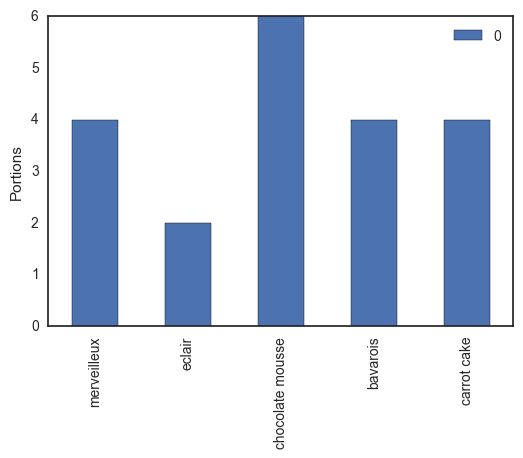
\includegraphics[scale=0.4]{chapters/assets/ot/desserts.png}
%     \caption{A distribution (histogram) of various sweets. If we mentally cut all these sweets into portions, we have twenty shares.}
%     \label{fig:ot-desserts}
% \end{figure}